% Figure for 02_datasets.qmd, copied from slides/AE_week01_Intro/AE_w01_intro.tex.
% Compile with pdflatex, then convert: pdftocairo -svg <name>.pdf ../<name>.svg
\documentclass[class=extarticle, 9pt, tikz, border=4pt]{standalone}
\usepackage[T1]{fontenc}
\renewcommand{\familydefault}{\sfdefault}
\definecolor{PelloGrayDark}{RGB}{60,60,60}
\definecolor{PelloGray}{RGB}{120,120,120}
\definecolor{PelloGrayLight}{RGB}{235,235,235}
\definecolor{PelloGrayUltraLight}{RGB}{248,248,248}
\begin{document}
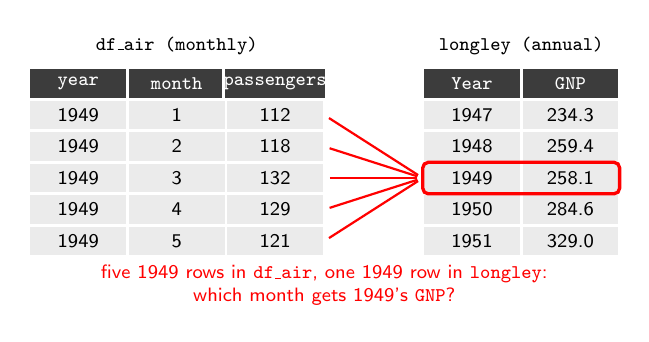
\begin{tikzpicture}[x=1.25cm, y=0.4cm, font=\scriptsize,
  cell/.style={draw=white, line width=1pt, fill=PelloGrayLight, minimum width=1.25cm, minimum height=0.4cm, inner sep=0pt},
  head/.style={cell, fill=PelloGrayDark, text=white, font=\scriptsize\ttfamily}]
  % table titles
  \node[font=\scriptsize\ttfamily] at (1,1.2) {df\_air (monthly)};
  \node[font=\scriptsize\ttfamily] at (4.5,1.2) {longley (annual)};
  % headers
  \node[head] at (0,0) {year};
  \node[head] at (1,0) {month};
  \node[head] at (2,0) {passengers};
  \node[head] at (4,0) {Year};
  \node[head] at (5,0) {GNP};
  % first five rows of each dataset
  \foreach \r/\v/\y/\g in {1/112/1947/234.3, 2/118/1948/259.4, 3/132/1949/258.1, 4/129/1950/284.6, 5/121/1951/329.0} {
    \node[cell] at (0,-\r) {1949};
    \node[cell] at (1,-\r) {\r};
    \node[cell] at (2,-\r) {\v};
    \node[cell] at (4,-\r) {\y};
    \node[cell] at (5,-\r) {\g};
    % every 1949 month points to the single 1949 row of longley
    \draw[red, thick, shorten <=2pt, shorten >=2pt] (2.5,-\r) -- (3.5,-3);
  }
  \draw[red, line width=1.2pt, rounded corners=2pt] (3.5,-2.5) rectangle (5.5,-3.5);
  \node[red, align=center] at (2.5,-6.4) {five 1949 rows in \texttt{df\_air}, one 1949 row in \texttt{longley}:\\ which month gets 1949's \texttt{GNP}?};
\end{tikzpicture}
\end{document}
